\section{Аналіз та вибір методів оцінювання та корекції в комплексній інерціально-супутниковій системі}

Основними задачами пілотажно-навігаційних комплексів (ПНК) як постачальника 
інформаційного забезпечення польоту ЛА є сумісна обробка навігаційної інформації, 
яка надходить на борт ЛА та забезпечення високої надійності функціонування бортових 
систем та комплексів ЛА і взагалі безпеки польоту за рахунок резервування 
джерел інформації. Висока ефективність використання інформації, яка 
надходить на борт ЛА, забезпечується застосуванням різних методів її обробки. 

Найкращі результати підвищення якісних характеристик вимірювальних комплексів 
досягаються  в системах зі структурною надмірністю, коли існує можливість 
отримання пілотажно-навігаційної інформації паралельно декількома способами з 
використанням інформації від приладів та вимірювальних систем, що входять до 
складу ПНК. Отримана таким чином інформація комплексується.

В існуючих ПНК широке розповсюдження знайшли такі способи сумісної обробки 
інформації, що надходять від декількох вимірників, як взаємна компенсація і 
фільтрація похибок вимірювальних приладів, що вимірюють один і той самий 
навігаційний параметр та оптимальне оцінювання вектора стану з використанням 
апріорної інформації про контрольований процес та поточні вимірювання.

Методи оптимальної обробки інформації в ПНК використовуються з метою 
отримання оцінок вектора стану повітряного судна (або деякої частини 
цього вектора) в умовах впливу випадкових збурень і завад на процес 
вимірювання. При цьому оцінюються не самі параметри польоту, а їхні похибки. 
За оптимальної обробки пілотажно - навігаційної інформації в ПНК найважливішим 
процесом є процес отримання оптимальних оцінок. В основу алгоритмів отримання 
оптимальних оцінок можуть бути покладені такі методи обробки інформації \cite{bib:pnk}:
\begin{itemize}
 \item метод найменших квадратів;
 \item метод максимуму правдоподібності;
 \item рекурентний неоптимальний фільтр;
 \item оптимальний фільтр Калмана.
\end{itemize}

\subsection{Огляд методів оптимальної обробки інформації}
Метод найменших квадратів (МНК) застосовується для одержання оптимальних оцінок при 
обробці накопичених вимірювань. Якщо виконано $m$ вимірювань координат $Х$ (параметрів) 
системи  $\dot{X}(t)=A(t)X(t)+B(t)u_{x}(t)$, тоді   
\begin{equation}
 Z = HX + Vz                                                                                                                                   \label{eq:sys_other_m}                                                                       
\end{equation}
\begin{ESKDexplanation}
\item де $H$ -- матриця спостереження;
\item $Z$, $X$ і $Vz$  -- вектори, компонентами яких є реалізація 
вектора вимірювання $Z$ i, вектора стану системи $X$ і вектора помилок 
вимірювання $Vz_{i}$  відповідно, причому $i=\overline{1,m}$.
\end{ESKDexplanation}
Необхідно за спостереженнями $Z$ і заданою матрицею спостереження $Н$ щонайкраще 
оцінити стан вектора $Х$. Критерієм такої оцінки за МНК служить функціонал 
$J= \sum _{i=1}^{m}V_{z_{i} }^{T}  V_{z_{i} } $
який  мінімізує  суму  квадратів  помилок  вимірювання   $Vz_{i}$.
У матричному виді цей вираз запишеться так:
\[J=|V_{z_{1} } V_{z_{2} } \ldots V_{z_{m} } |\left|
\begin{array}{c} {V_{z_{1} } } \\ 
{V_{z_{2} } } \\ 
{\vdots } \\ 
{V_{z_{m} } } 
\end{array}\right|\] 
або з урахуванням \eqref{eq:sys_other_m} 
\begin{equation}
J = (Z - HX)^{T}(Z - HX)                                                    
\label{eq:__1_16_}
\end{equation}
Оцінку $\hat{X}$, вектора стану системи $Х$ можна одержати 
шляхом розв'язання  рівняння  $\frac{\partial J}{\partial X} =0$.

З урахуванням рівняння \eqref{eq:__1_16_} маємо

\begin{equation} 
\label{eq:solve_rms_} 
H^{T} (Z-H\hat{X})+(Z-H\hat{X})^{T} H=0 
\end{equation} 

Доданки виразу \eqref{eq:solve_rms_} рівні між собою, оскільки є добутками транспонованих 
відносно один до одного однакових співмножників $H$ і ($Z- H\hat{X }$). 
Отже, тільки рівність  нулю кожного з цих двох доданків забезпечує 
рівність нулю виразу \eqref{eq:solve_rms_}.
Отже                   
\[ H^{T}(Z-H \hat{X}) = 0 \]
Відтепер можна сформулювати необхідні і достатні умови одержання оптимальних оцінок $\hat{X}$
вектора стану системи $Х$ за методом найменших квадратів  
у вигляді основних положень, виконання яких передбачає:
\begin{itemize}
\item наявність накопичених спостережень $Zi$, $i=\overline{1,m}$;
\item знання матриці спостережень $Н$;
\item не особливість матриці $H^{T}$ $H$, тобто $H^{T}$ $H \ne 0$.
\end{itemize}

% \includegraphics[bb=0mm 
% 0mm 208mm 296mm, width=148.7mm, height=47.1mm, viewport=3mm 4mm 205mm 292mm]{image6.eps}Структурна 
% схема одержання оптимальних оцінок за методом найменших квадратів показана на рис.1.9    
% Рис.1.9 
% Структурна схема одержання оптимальних оцінок за МНК
Отримання оцінки  $\hat{X}$  зв'язано з накопиченням спостережень  $Zm$  
у наслідок чого нова оцінка параметра не збігається за часом з його поточним значенням 
на час, необхідний для накопичення спостережень. Тому даний алгоритм для оцінки використовують 
лише у випадку виміру того самого параметра одночасно кількома датчиками.

Метод найменших квадратів застосовується в тому випадку, коли надлишок інформації 
виходить за рахунок рівно точних вимірювань різними датчиками інформації. При цьому, 
вимоги щодо спектрального складу помилок датчиків не відзначаються. Відповідно до 
цього методу, має місце мінімізація суми квадратів помилок всіх вимірювань. \\

\textit{Алгоритм оцінювання за методом максимуму правдоподібності}\\

Алгоритм оцінювання за методом максимуму правдоподібності  як і алгоритм оцінювання 
за МНК потребує накопичення вимірювань, тобто наявності вектора спостережень.
Передбачається, що похибки вимірювання розподілені за нормальним законом. Тоді щільність 
розподілу ймовірностей вектора  $Vz_m$ має вигляд:
\begin{equation}
P\left(V_{z_{m} } \right)=\frac{1}{\sqrt{(2\pi)^{m} \left|R_{z} \right|} 
} {\rm exp}\left[-\frac{1}{2} V_{z_{m} }^{T} R_{z}^{-1} V_{z_{m} } \right],                       
\label{eq:solve_mle}
\end{equation}
\begin{ESKDexplanation}
\item де $R_z$ -- кореляційна матриця похибок вимірювання; 
\item $|R_z|$ -- визначник матриці $R_z$.                                                   
\end{ESKDexplanation}
Використання алгоритму оцінок за методом максимуму правдоподібності передбачує виконання умови 
$|R_z|\neq 0$, тобто матриця $R_z$ не повинна бути 
особливою. Підставивши \eqref{eq:sys_other_m} у \eqref{eq:solve_mle}, отримаємо 
вираз для функції правдоподібності.

\[\psi (X)=\frac{1}{\sqrt{(2\pi )^{m} \left|R_{z} \right|} } exp \left[-\frac{1}{2} 
(Z_{m} -HX_{m} )^{T} R_{z}^{-1} (Z_{m} -HX_{m} )\right],\] 
яка являє собою щільність розподілу помилок  вимірювання.

Необхідно обрати таку оцінку  $\hat{X}_{m}$, при якій функція 
правдоподібності $ \psi$(Х) перетворюється в максимум, що відповідає 
мінімуму квадратів відхилень виміряних координат вектора $X$ від їхнього дійсного значення. 
Для цього необхідно, щоб $\frac{\partial \psi (X)}{\partial X} =0$.

На практиці зручніше обчислювати максимум не самої функції правдоподібності, a її 
логарифма, тобто 
\begin{equation}
Ln \psi (X)= Ln\frac{1}{\sqrt{(2{\rm 
\pi })^{m} \left|R_{z} \right|} } -\frac{1}{2} (Z_{m} -HX_{m} )^{T} R_{z}^{-1} 
(Z_{m} -HX_{m} ).       
\label{eq:__1_18_}
\end{equation}
Узявши в рівнянні \eqref{eq:__1_18_} похідні за компонентами вектора $Xm$ 
і прирівнюючи їхню суму до нуля, одержимо:
\begin{equation}
\frac{1}{2} H^{T} R_{z}^{-1} (Z_{m} -H\hat{X}_{m} )+\frac{1}{2} 
HR_{z}^{-1} (Z_{m} -H\hat{X}_{m} )^{T} =0              
\label{eq:__1_19_}
\end{equation}
Зауважимо, що як і для формули оцінки вимірювань за методом найменших квадратів, один із доданків 
виразу \eqref{eq:__1_19_} є транспонованим відносно іншого. Отже, доданки цього 
виразу рівні між собою, вони не можуть бути від'ємні, тому кожний з них дорівнює 
нулю. 

Припустимо, що      
\[ H ^{T} R_{z}^{-1} (Z_{m} -H\hat{X}_{m} )=0 \]
тоді   
\begin{equation}
\hat{X }_{m} =(H^{T} R_{z}^{-1} H)^{-1} H^{{\rm T}} R_{z}^{-1} Z_{m} 
\label{eq:solve_mle_end}
\end{equation}
Вираз \eqref{eq:solve_mle_end} стає вихідним для розробки алгоритму отримання оптимальних 
оцінок  за методом максимуму правдоподібності.

Для визначення цих оцінок необхідно:
\begin{itemize}
\item накопичити m  спостережень -- $Zm$;
\item знати кореляційну матрицю $Rz$ похибок вимірника;
\item знати матрицю зв'язків спостереження $H$.
\end{itemize}

% \includegraphics[bb=0mm 0mm 208mm 296mm, width=162.4mm, height=55.0mm, viewport=3mm 
% 4mm 205mm 292mm]{image7.eps}Структурна схема отримання оптимальних оцінок за методом 
% максимуму правдоподібності показана на рис.1.10
% Рис.1.10 Структурна схема отримання оптимальних оцінок за методом максимуму правдо 
% подібності
Як і для алгоритму оцінок за МНК отримання оцінки $\hat{X}_{m} $  пов'язано 
з накопиченням вимірювань $Zm$, тому цей метод, як і МНК, можна використовувати 
лише при вимірюванні одного параметра декількома системами. В іншому випадку нова 
оцінка помилок ПНК не буде співпадати з поточним значенням помилок на час, що дорівнює 
часу накопичення спостережень.

Алгоритм оцінювання за методом максимуму правдоподібності, як і алгоритм оцінювання 
за методом найменших квадратів, потребує накопичення вимірювань, тобто наявності 
вектора спостережень. Цей метод пропонує максимізацію функції правдоподібності, що 
відповідає мінімуму квадратів помилок. При цьому, передбачається, що похибки вимірювання 
розподілені за нормальним законом.\\

\textit{Рекурентний метод обробки інформації } \\

Рекурентний метод обробки інформації дозволяє отримати оцінку параметра після кожного 
досліду. За результат оцінки вимірюваного параметра $х_m$ при проведенні m спостережень 
візьмемо:          
\[ \hat{x}_{m} =\frac{1}{m} \sum _{i=1}^{m}z_{i},\]
\begin{ESKDexplanation}
\item де $z_{i} =x+v_{z_{i}}$, $i=\overline{1,{\rm \; }m}$; 
\item x -- вимірюваний параметр; 
\item $v_{z_{i}}$ -- похибка i-го спостереження.
\end{ESKDexplanation}

Тоді на черговому $(i + 1)$-му кроці вимірювань значення оцінки $\hat{x}_{m+1} $, 
має вигляд:
 \begin{equation} 
\hat{x}_{m+1} =\frac{\left(\sum _{i=1}^{m}z_{i}  \right)+z_{m+1}}{m+1} 
=\frac{m}{m+1} \left(\frac{1}{m} \sum _{i=1}^{m}z_{i}  \right)+\frac{1}{m+1} 
z_{m+1}            
\label{eq:__1_21_}
\end{equation}
або 
\[ \hat{x}_{m+1} =\frac{m}{m+1} \hat{x}_{m} +\frac{1}{m+1} z_{m+1}\].
де $z_{m+1}$ -- останнє (m +1)-ше спостереження.

Виконавши певні перетворення отримаємо:
\[\hat{x}_{m+1} =\hat{x}_{m} +\frac{1}{m+1} \left(z_{m+1} 
-\hat{x}_{m} \right)\] 
або, позначивши  $\frac{1}{m+1} =k$,    
\begin{equation} 
\label{eq:solve_recurs} 
\hat{x}_{m+1} =\hat{x}_{m} +k\left(z_{m+1} -\hat{x}_{m} \right). 
\end{equation} 

Отже, оцінку $\hat{x}_{m+1} $ можна отримати з попередньої оцінки$\hat{x}_{m} $ шляхом 
складання її з різницею між новим  спостереженням zm+1 та попередньою оцінкою, помноженою  
на коефіцієнт ваги \textit{k}. У цьому випадку зникає необхідність зберігати m спостережень, 
отриманих на попередніх кроках вимірювання, оскільки вся попередня інформація об`єднана 
в апріорній оцінці $\hat{x}_{m} $. 

% Математична модель рекурентного методу 
% обробки інформації показана на рис1.11

% \includegraphics[bb=0mm 0mm 208mm 296mm, width=164.4mm, height=52.2mm, viewport=3mm 
% 4mm 205mm 292mm]{image8.eps}
% 
% Рис.1.11 Математична модель рекурентного методу обробки інформації 
Рекурентний алгоритм \eqref{eq:solve_recurs} зв`язує поточне значення оцінки $\hat{x}_{m+1} $ з 
її попереднім значенням $\hat{x}_{m} $

Різниця  ($z_{m+1} -\hat{x}_{m} $) стає показником  цінності 
інформації, яку отримують при проведенні $z_{m+1}$ -го спостереження. Дійсно, 
якщо ця різниця близька до нуля, то зафіксоване спостереження $z_{m+1}$ не несе 
будь-якої нової інформації у порівнянні з апріорною, і в цьому випадку 
$\hat{x}_{m+1} \cong \hat{x}_{m} $. Навпаки, при великій різниці  
($z_{m+1} - \hat{x}_{m} $) з урахуванням вагового коефіцієнта здійснюється суттєве уточнення 
оцінки  $\hat{x}_{m} $,  отриманої на попередньому кроці розрахунків. 

Але коефіцієнт  $k=\frac{1}{m+1} $ отримано без використання критерію  оптимальності, 
тому оцінка $\hat{x}_{m+1} $ також не є оптимальною, що знижує цінність 
даного методу обробки інформації.

Алгоритм неперервного оптимального фільтра Калмана об'єднує розв'язання двох задач: 
спостереження та фільтрації , враховуючи характеристики контрольованого процесу, 
мінімізує помилку оцінювання. З іншого боку ФК дозволяє оцінити навігаційні параметри, що
безпосередньо не спостерігаються, а відносна простота реалізації алгоритму в БЦОМ робить цей метод комплексної обробки інформації найбільш привабливим. Детальніше алгоритм роботи, розглянемо в наступному розділі.

\subsection{Рекурентний фільтр Калмана}

Оптимальний фільтр Калмана \cite{bib:kalman_1} — ефективна і гнучка процедура для комплексної обробки інформації із зашумлених 
датчиків для оцінки стану стохастичної системи. В більшості випадків, кількість параметрів, що задають стан об’єкту, більше, ніж
кількість спостерігаємих параметрів, доступних для вимірювання. За допомогою моделі об’єкту по ряду доступних вимірів фільтр Калмана
дозволяє отримати оцінку внутрішнього стану системи.

ФК -- призначений для рекурсивного дооцінювання вектора стану апріорно відомої динамічної системи, для розрахунку
поточного стану стану системи необхідно знати поточні виміри, а також попередній стана самого фільтра. Таким чином фільтр Калмана,
як і інші рекурсивні фільтри, реалізований в часовому представленні, а не в частотному.

Фільтра включає 2 типа змінних:
\begin{enumerate}
 \item Вектор стану системи, включає наступні компоненти:
  \begin{itemize}
    \item Змінні, які безпосередньо нас цікавлять (необхідно знайти, наприклад швидкість, прискорення)
    \item Змінні, які безпосередньо не використовуються, але необхідні для процесу оцінювання. 
    В загальному випадку не важливо знати їхні значення, але необхідно визначити їх для для 
    покращення точності оцінки.
    \item Фільтр Калмана у специфічних задача має включати всі ті змінні динаміки системи, які можуть 
    бути виміряні ДПІ.
    \end{itemize}
 \item Коваріаційна матриця: міра невизначеності оцінювання. Рівняння, що використовуються для 
отримання коваріаційної матриці ( рівняння Рікатті) та управління невизначеністю, визначають 
як шум датчиків та динаміка невизначеності впливають на невизначеність стану системи, що оцінюється.
\end{enumerate}

За допомогою отримання невизначеності власне системи і невизначеності у відповідних 
показника датчиків, ФК дає можливість комплексувати данні з усіх ДПІ “отимально”, в 
сенсі, що результуюча оцінка мінімізує квадратичну функцію помилки оцінки, включаючи 
мінімальне середньо квадратичне відхилення будь-якої лінійної комбінації помилок оцінювання. 
Коефіцієнт підсилення Калмана — оптимальна зважена матриця, що поєднує данні ДПІ з попередньою 
оцінкою, для отримання нової апостеріорної оцінки.\\


\textit{Рівняння динамічної системи}\\

Фільтр Калмана намагається оцінити стан змінної $x\in \Re^{n}$ дискретно управляємого
процесу, що описується лінійними стохастичними диференціальним рівняннями:
\begin{equation}
\label{eq:linear_sys}
x_{k} = \Phi x_{k-1} + w_{k-1},
\end{equation}
З вимірюваннями  $Z\in \Re^{m}$:
\begin{equation}
\label{eq:linear_sys_measure}
z_{k} = Hx_{k} +v_{k},
\end{equation}

Випадкові змінні $w_{k}$ та $v_{k}$ представляють шум системи (process noise) та 
шум вимірювань (measurement noise), які вважаються незалежними один від одного,
білими з нормальним розподілом шумами.
\begin{eqnarray} 
\label{eq:pw} p(w)\sim N(0,Q), \\
\label{eq:pv} p(v)\sim N(0,R).
\end{eqnarray} 
На практиці, коваріаційна матриця шуму системи $Q$ та коваріаційна
матриця шуму вимірювань $R$ можуть змінюватись на кожному кроці вимірювань,
але для простоти, в нашому випадку, вони постійні.

Матриця $\Phi$ розміром $n \times n$ в диференціальному рівнянні \eqref{eq:linear_sys}
проводить залежність між попереднім станом системи $k-1$ та поточним станом
$k$, при наявності вхідного сигналу чи шуму. Матриця \textbf(H) $m \times n$ в 
рівнянні \eqref{eq:linear_sys_measure} відповідає вимірюванням $z_{k}$. \\

\textit{Отримання рівнянь фільтра}\\

Позначимо $\hat{x}(-) \in \Re^{n}$ --- апріорна оцінка на кроці $k$ 
інформація про рух системи до кроку $k$, та $\hat{x}(+) \in \Re^{n}$
апостеріорна оцінка на кроці $k$ за допомогою вимірювань $z_{k}$. 
Відповідно апріорна оцінка коваріації помилки:
\begin{equation}
\label{eq:p_minux}
P_{k}(-)= E[(x_{k}-\hat{x}_{k}(-))(x_{k}-\hat{x}_{k}(-))_{T}]
\end{equation}
та апостеріорна коваріаційна матриця помилок:
\begin{equation}
\label{eq:p_plus}
P_{k}(+)= E[(x_{k}-\hat{x}_{k}(+))(x_{k}-\hat{x}_{k}(+))_{T}]
\end{equation}

При виведенні рівнянь фільтра Калмана, наша ціль -- знайти рівняння, що 
розраховують апостеріорну оцінку стану $\hat{x}_{k}(+)$ як лінійну компенсацію
апріорної оцінки стану $\hat{x}_{k}(-)$ та взваженої різниці між безпосередньо
вимірами $z_{k}$ та їхнім прогнозом $H\hat{x_{k}}$, як показано нижче \eqref{eq:k_update}
\begin{equation}
  \label{eq:k_update}
 \hat{x}_{k}(+)= \hat{x}_{k}(-) + K\left[z_{k}-H\hat{x}_{k}(-)\right]
\end{equation}
Різниця $(z_{k}-H\hat{x}_{k}(-))$  -- називається інноваціями (\textit{innovation}) 
або залишками (\text{residual}). Залишки, як відображення дисперсії між прогнозованими
вимірами $H\hat{x}_{k}(-))$ та безпосередніми вимірами $z_{k}$. Залишок, який
рівний нулю, означає, що обоє вимірів знаходяться в повному узгодженні.

Матриця $K$ $n \times m$ визначає коефіцієнт підсилення або фактор
змішування, який мінімізує апостеріорну помилку оцінки \eqref{eq:p_plus}.
Мінімізація може бути закінчена підстановкою \eqref{eq:k_update} у подане 
вище визначення для коваріації \eqref{eq:p_plus}, виконуючи необхідні дії та
взявши похідну по $K$, встановивши результат рівним нулю, а потім
вирішуючи відносно $K$ рівняння. Детальне виведення рівнянь описане в \cite{bib:gps_ins}.
Результат може бути отриманий в наступній формі:
\begin{equation}
  \label{eq:k_gain}
  K_{k}=P_{k}(-)H^{T}(HP_{k}(-)H^{T}+R)^{-1} = \frac{P_{k}(-)H^{T}}{HP_{k}(-)H^{T}+R} 
\end{equation}
Зважаючи на \eqref{eq:k_gain}, якщо коваріаційна матриця помилок вимірювання
$R$ прямує до нуля, коефіцієнт підсилення $K$ взважує залишки 
більш сильно.Наприклад:
\begin{equation}
  \label{eq:lim_R}
  \displaystyle\lim_{R_{k}\to 0} K_{k} = H^{-1}
\end{equation}
Якщо апріорна оцінка коваріаційної матриці $P_{k}(-)$ наближається
до нуля, коефіцієнт підсилення $K$ майже не взважує залишки.
\begin{equation}
  \label{eq:lim_P_minus}
  \displaystyle\lim_{P_{k}(-)\to 0} K_{k} = 0
\end{equation}

З іншого боку, взважування за допомогою $K$, у випадку коли коваріація 
помилки вимірювань $R$ наближається до нуля, то безпосереднім вимірам
$z_{k}$ довіряється все більше і більш, коли прогнозовані виміри $H\hat{x}_{k}(-))$
враховуються все менше. Але якщо апріорна коваріація помилки $P_{k}(-)$ наближається
до нуля то спостерігання $z_{k}$ майже не враховуються, коли відповідно
прогнозовані виміри $H\hat{x}_{k}(-)$ стають більш ``впливовими''.

\subsection{Алгоритм фільтра Калмана}

ФК знаходить стан системи за допомогою форми зворотнього зв'язку: фільтр
оцінює стан процесу в один момент часу, а потім отримує зв'язок в формі
зашумлених вимірів. Такі рівняння для фільтра розділяються на дві групи: 
прогноз та корекція на основі вимірів. Прогноз відповідає за екстраполяцію
в часі поточного стану системи та її коваріації для отримання апріорної
оцінки для наступного кроку. Рівняння корекції необхідні для зворотнього
зв'язку -- використовують нові виміри і апріорні оцінки для отримання 
апостеріорних оцінок.

Для фільтра не важливо з якого кроку починати, так і рівняння можуть бути 
представлені з точки зору прогнозу та корекції Рис.\ref{fig:basic_cycle}
\begin{figure}[here]
\centering
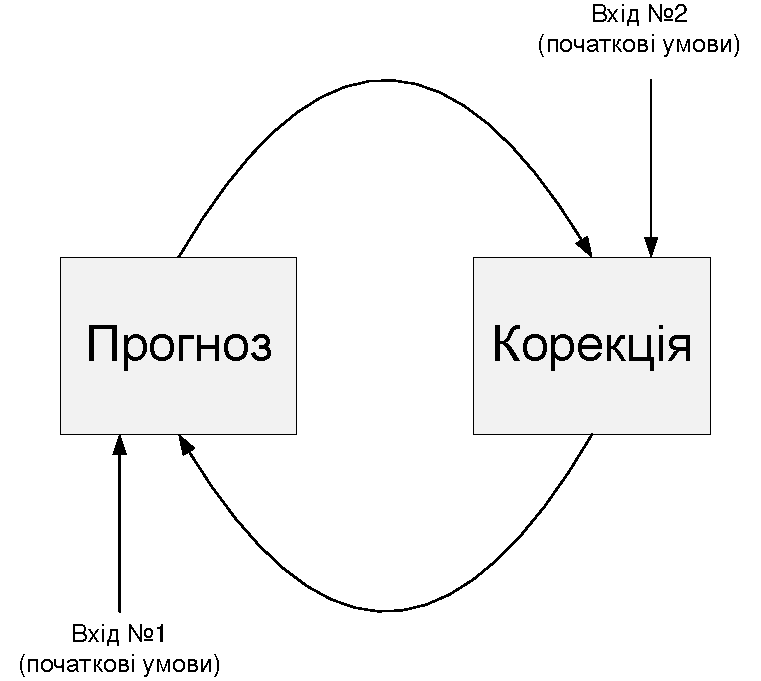
\includegraphics[scale=0.55]{pre_upd}
\caption{Цикл функціонування фільтра Калмана }
\label{fig:basic_cycle}
\end{figure} 

\begin{table}[here]
\small
\caption{Рівняння дискретного фільтра Калмана}
\centering
\begin{tabular}{|p{160mm}|} \hline 


Рівняння / Формула \\ \hline 
\begin{eqnarray} 
% \begin{array}{cc}
\text{Модель динаміки системи}  &  \label{eq:kalman_1} x_{k} = \Phi x_{k-1} + w_{k-1}, \\  
\text{Модель вимірювань}  & \label{eq:kalman_2} z_{k} = Hx_{k} +v_{k} \\ 
\text{Початкові умови}  &\label{eq:kalman_3} E[x_{o}] = \hat{x}_{0}, E[x_{o} x_{o}^{T}] = P_{0} \\
\text{Припущення незалежності}  &  \label{eq:kalman_4} E[w_{k} v_{j}^{T}] = 0 \text{для всіх k та j} \\
\text{Екстраполяція оцінки (прогноз)}  &  \label{eq:kalman_5} \hat{x}_{k}(-) = \Phi \hat{x}_{k-1}(+)\\
\text{Екстраполяція коваріації}  &  \label{eq:kalman_6} P_{k}(-) = \Phi_{k-1} P_{k-1}(+)\Phi_{k-1}^{T} + Q_{k-1} \\ 
\text{Корекція оцінки}  &  \label{eq:kalman_7} \hat{x}_{k}(+) = \hat{x}_{k}(-) + K_{k}[z_{k}-H_{k}\hat{x}_{k}(-)]\\
\text{Корекція оцінки коваріації}  &  \label{eq:kalman_8} P_{k}(+) = [I - K_{k}H_{k}]P_{k}(-)\\
\text{Коефіцієнт підсилення Калмана}   &  \label{eq:kalman_9} K_{k}= P_{k}(-)H_{k}^{T}[H_{k}P_{k}(-)H_{k}^{T} + R_{k}]^{-1}  
% \end{array}
\end{eqnarray} 
\\  \hline
\end{tabular}
\label{tb:ac}
\end{table}
Перше завдання при корекції -- розрахувати коефіцієнт підсилення Калмана, $K_{k}$/
Наступний крок, безпосередньо отримати виміри $z_{k}$, а потім генерувати 
апостеріорну оцінку за допомогою \eqref{eq:k_update}. Останній крок  -- це 
отримання апостеріорної коваріаційної матриці оцінки помилки.

Після кожного разу екстраполяції та корекції, процес повторюється, попередні
апостеріорні оцінки використовуються для прогнозу нових апріорних оцінок.
Ця рекурсивна природа є найбільш важливою особливістю фільтра Калмана, це робить
його більш практичним, в порівнянні з іншими фільтрами (наприклад фільтр Віннера)
\begin{figure}[here]
\centering
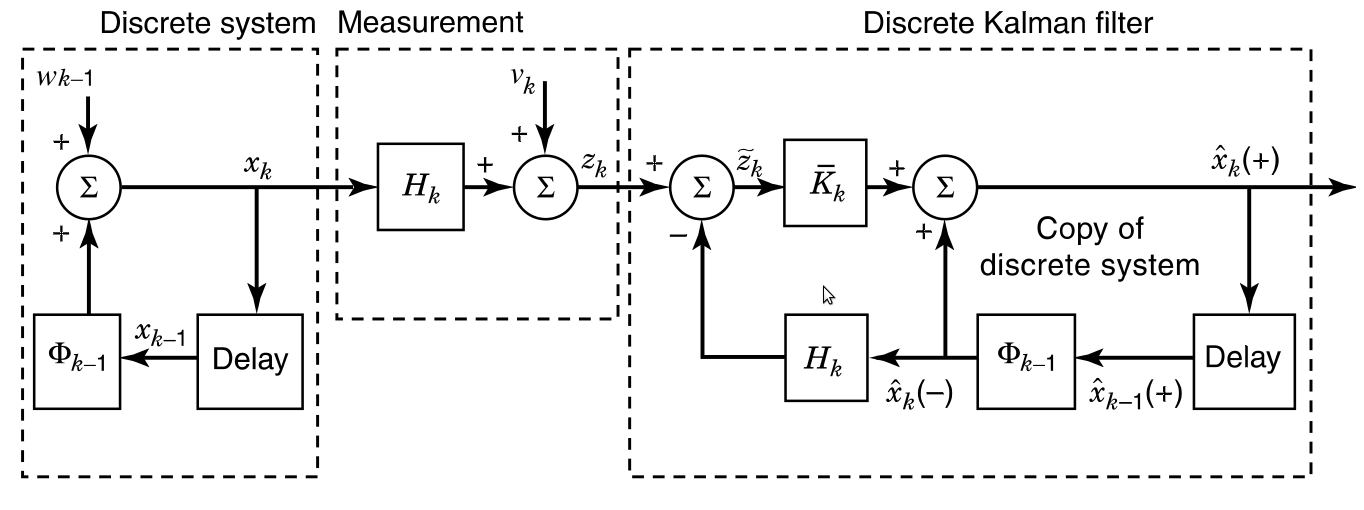
\includegraphics[scale=0.35]{kalman_flow}
\caption{Блок діаграма системи, моделі вимірювань та дискретного ФК}
\label{fig:kalman_flow}
\end{figure} 

\subsection{Проектування фільтра Калмана}

В практичній реалізації фільтра, коваріація вимірюваного шуму $R$ вимірюється
звичайно до використання фільтра. Знаходження цієї матриці в загальному випадку
практична задача, виміряні величини дають можливість визначити дисперсію шуму, що
діє на данні датчиків.

Визначення коваріації шуму системи $Q$ в загальному більш складна задача,
просто не має можливості безпосередньо спостерігати процес який оцінюється.
Інколи відносно проста модель процесу може дати прийнятний результат, якщо
введена достатня величина невизначеності процесу через вибір матриці $Q$.

В іншому випадку, є чи немає раціональної бази для вибору параметрів, часто
краща продуктивність (з точки зору статистики) може бути отримана за допомогою
налаштування параметрів фільтра $Q$ та $R$. 

Асиметрія коваріаційної матриці $P$ один з факторів, що впливає на чисельну
нестійкість рівняння Рікатті. Якщо не використовується фільтр з квадратним
коренем, тоді ця матриця може бути ``симетризована'' просто за наступною 
формулою:
\begin{equation}
 \label{P_symetry}
P= \frac{1}{2}(P+P^{T})
\end{equation}
Цей метод використовується протягом довгого часу і добре себе зарекомендував.

При проектуванні фільтра, корекція коваріаційної матриці \eqref{eq:kalman_6} та
\eqref{eq:kalman_8} має бути перевірена не тільки на симетрію але й на 
додатно визначеність.
Якщо ці умови не будуть виконуються, це свідчить про помилки в програмі або
матриця погано обумовлена. Для усунення проблеми обумовленості використовується
інше рівняння для $P_{k}(+)$, яке називається формою Джозефа \cite{joseph}, яка показна на
наступному рівнянні:
\begin{equation}
 \label{P_plus_Joseph}
P_{k}(+)=[I-K_{k}H_{k}]P_{k}(-)[I-K_{k}H_{k}]^{T}+K_{k}R_{k}K_{k}^{T}
\end{equation}
З рівняння видно, що права частина є сумою двох симетричних матриць.
Перша додатно визначена інша не від'ємно визначена, що робить $P_{k}(+)$ 
додатно визначеною матрицею.

Безперечно саме фільтр Калмана найбільш привабливий при розв’язанні задачі 
комплексної обробки інформації в інерціально-супутникових системах навігації. 
